\chapter{Hardware design}
\head{This chaper describes the design considerations that has been thought of whilst designing a about 1 metre boat for this project.}

\section{LLI electronics}
The \ac{LLI} electronics should be a kind of plug and play device that can be put into serval smaller ship designs. It should provide outputs to control different kind of actuators, and it should also provide basic sensor readings to the \ac{HLI} and \ac{GRS}, whilst being able to have a few general IO pins to miscellaneous stuff.

The \ac{LLI} has been designed to allow for the mentioned functionality. As described in section~\vref{sec:platform} the \ac{LLI} is an embedded platform. In this case a Atmel AVR microcontroller has been choosen. The electronics/hardware used in this case is an Arduino Mega 2560, where a shield to interface all peripehals has been designed. The schematic for this can be seen in appendix~\vref{chap:schema}.

It has been designed as a box with the following features:
\begin{description}
\item[Serial]\hfill \\ interface supposed to be used to the \ac{HLI} with a baud rate of 115200 bps
\item[PWM]\hfill \\ outputs for actuators. Both some PWM outputs supposed to be used with servos and \ac{ESC}'s used in RC hobby, together with some full range and kilo hertz range frequencies, which could be used for modulating H-bridge drivers directly.
\item[I$^2$C]\hfill \\ option for aux communication \todo{hmm, maybe I actually forgot to wire this to the interface connector}
\item[Analog]\hfill \\ inputs which could be used for i.e. temperature sensors.
\item[Relay driver]\hfill \\ output, i.e. to cutoff actuator power.
\item[5V]\hfill \\ regulated output.
\end{description}

The hardware layout can be seen in figure~\vref{fig:lli-hw} and the hardware schematic can be seen in appendix~\vref{chap:schema}.



\section{Bow thruster}
The ship design includes a bow thruster, which can be used to perform precision maneuvers in tight spaces. This component is not currently included in our control algorithms, because it has little or no effect on the ship when used at speeds above \todo{what speeds?}. It will be controlled by the \ac{LLI} with a direction and a \ac{PWM} signal. 

The electronic design of the bow thruster controller can be found in subsection \ref{subsec:bow thruster controller}: Bow thruster controller.

\section{Ship hull}

The hull of the ship follows a soft-chined displacement design, because in normal operating conditions the static buoyancy will dominate over dynamic. This shape affected less by the currents of the sea, and more by the wind. According to the data series of the British Oceanographic Data Centre\footnote[1]{https://www.bodc.ac.uk/data/online$\_$delivery/nodb/search/} near the shores of Greenland the drift caused by the steady currents is generally higher than the wind with a more randomly distributed blowing direction.

\begin{figure}[hullshape]
	\centering
	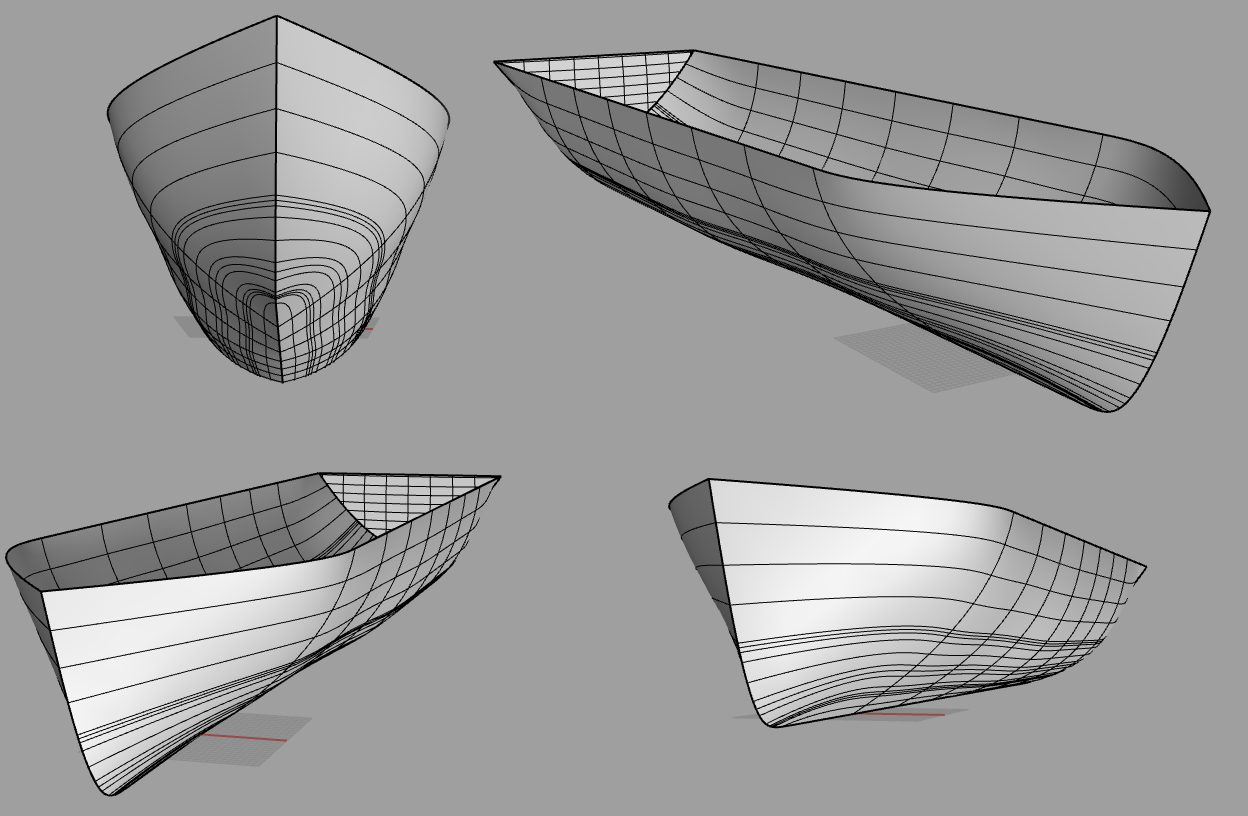
\includegraphics[width=\textwidth]{img/render/rendermontage.png}
	\caption{The shape of the hull}
	\label{fig:vessel-block-overview}
\end{figure}

The ship is outfitted with powerful main engines, so the vessel can perform fast and precise maneuvering without the bow thruster. Though these engines provide a lot of dynamic range, the ship hull was not designed for high speed \ref{jumping}. The problem is caused by the size and power of the propellers. At slower speeds the effect ceases \ref{jumping}.
Mirroring the setup and reversing the rotation movement would solve the pushing problem, but instead the back of the ship is pushed upwards, and air is sucked between the propellers. Instead, an additional vertical fin has been installed above the propellers, which keeps the water from being pushed upwards. As a positive side effect, the water after the hull is significantly less disturbed, thus the drag has been reduced as well. This has a positive effect on the range through the battery life \ref{fin}.

\begin{figure}[jumping]
	\centering
	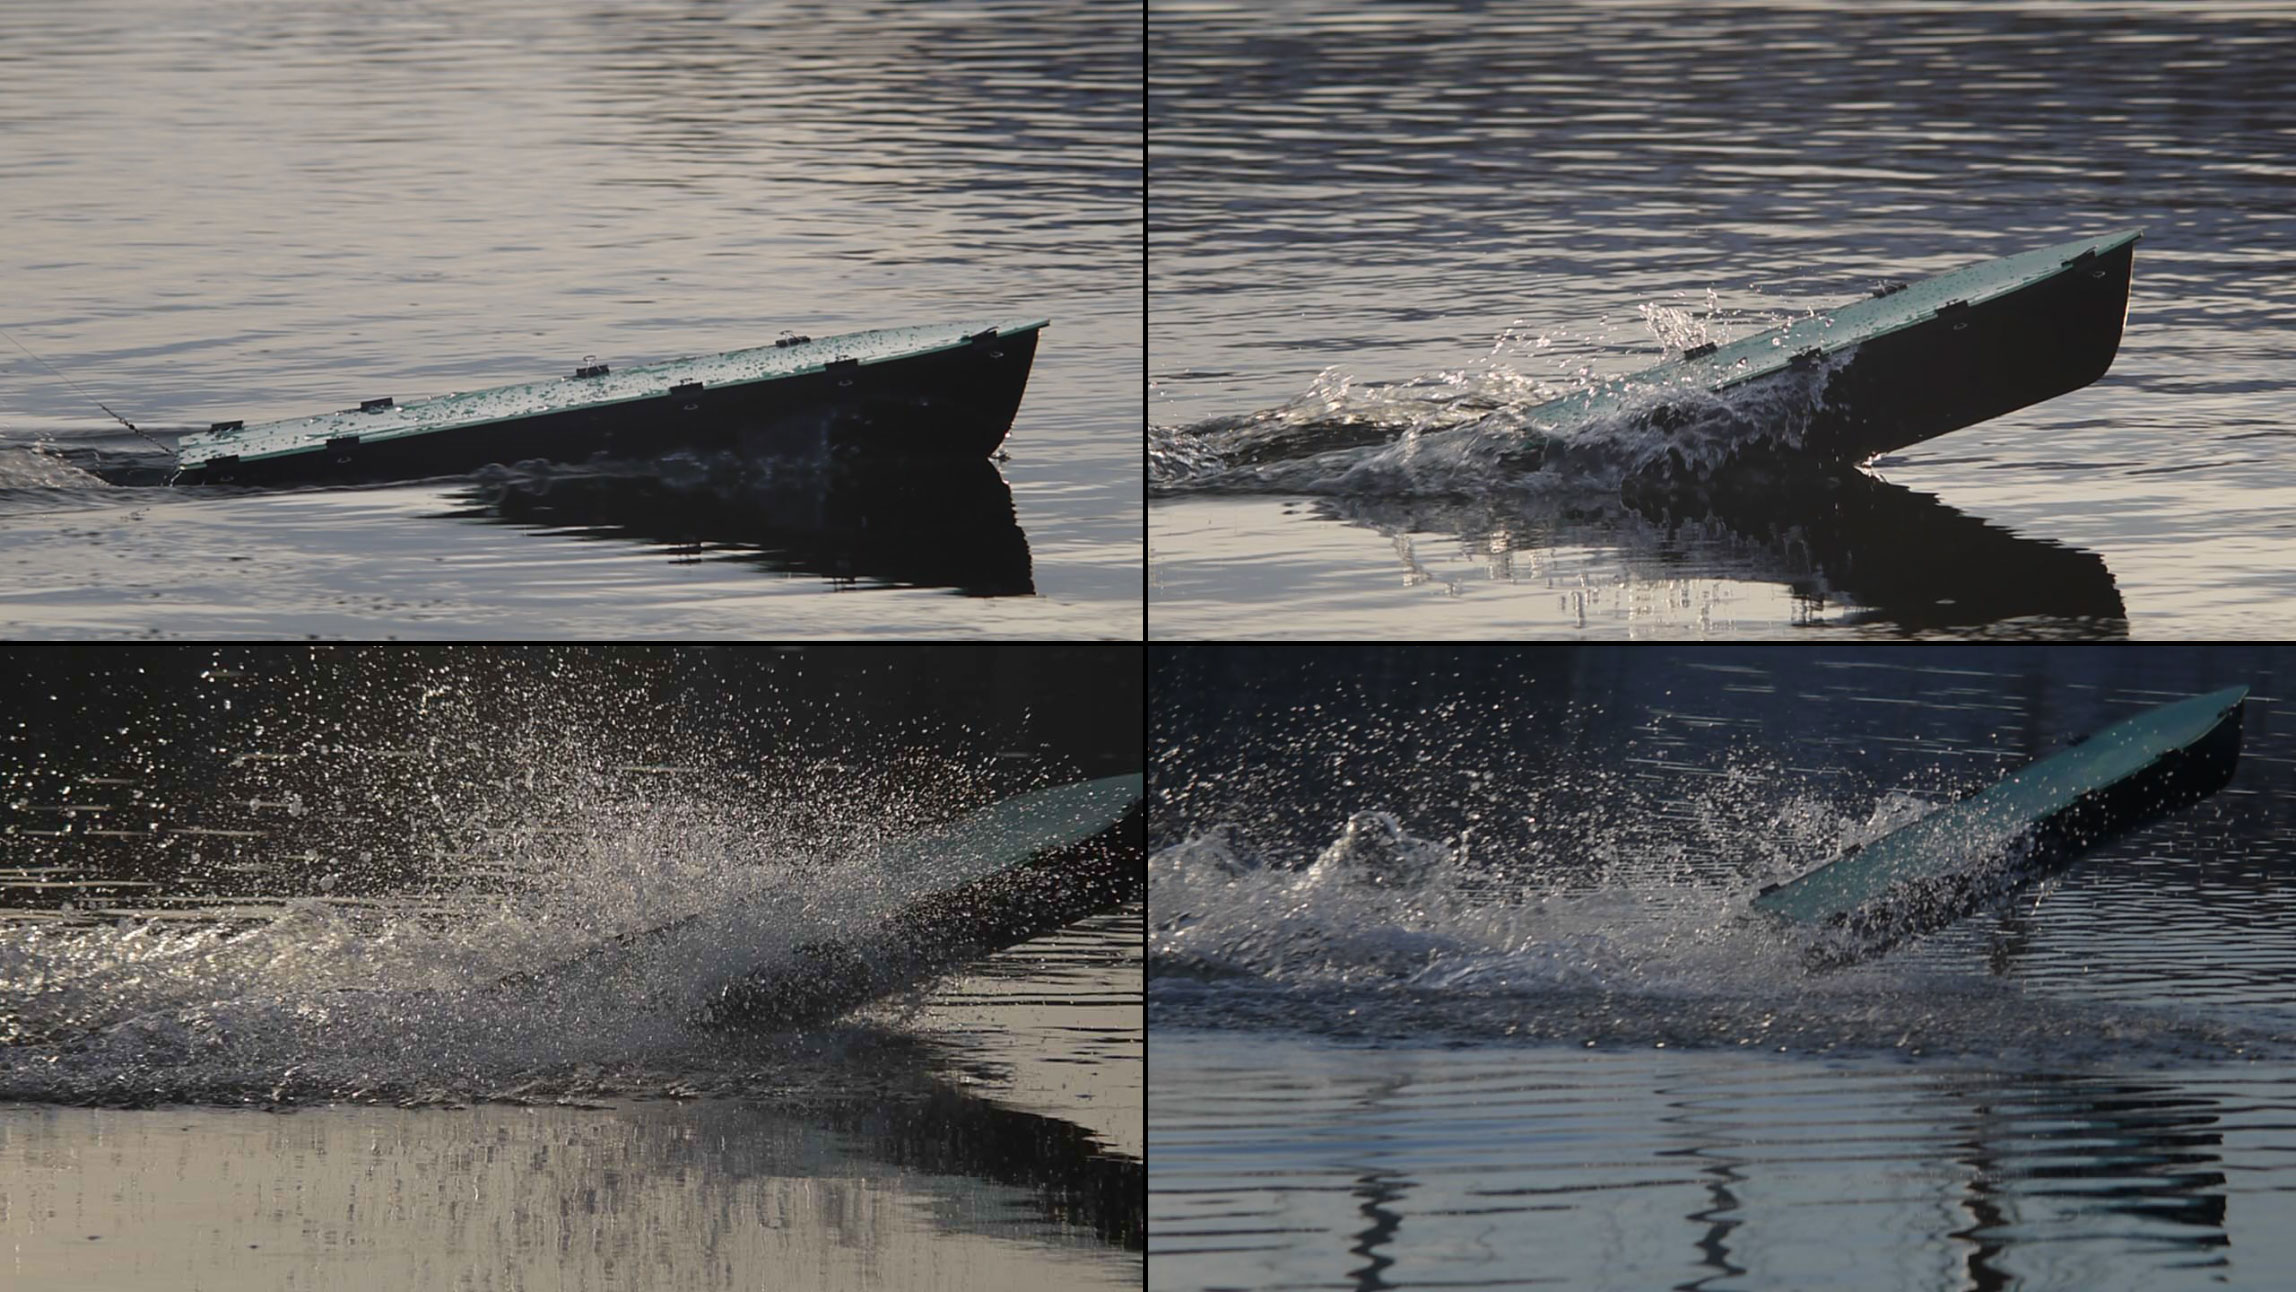
\includegraphics[width=\textwidth]{Pictures/VerticalJumpingTele.jpg}
	\caption{An excessive and unregulated bouncing can be experienced at high speeds.}
	\label{fig:vessel-block-overview}
\end{figure}

\begin{figure}[waterpushup]
	\centering
	\includegraphics[width=\textwidth]{Pictures/Forward.jpg}
	\caption{The power of the two engines force the water upwards between the propellers, therefore pushing the back of the ship down}
	\label{fig:vessel-block-overview}
\end{figure}

\begin{figure}[fin]
	\centering
	\includegraphics[width=\textwidth]{Pictures/Fin.jpg}
	\caption{The rotating propellers with the fin mounted above them. The engine power is set in the normal operation range}
	\label{fig:vessel-block-overview}
\end{figure}